\documentclass{jpreprint}
\usepackage{setspace}
\usepackage{amsmath}
\usepackage{subfig}
\usepackage{float}

\def\vector#1{\mbox{\boldmath{$#1$}}}

\jtitle{
コード進行および歌詞情報を用いた\\
楽曲分類システムの構築
}
\title{
Construction of Musical Compositions Classification Systems \\
Based on Chord Progressions and Lyrics
}
\jauthor{齋藤 佑樹}
\author{Yuki Saito}
\jcourse{電子情報システム工学専攻}
\course{Electronic and Information Systems Engineering}
\jlab{天元} % 研究室名(指導教員名)
% 以下の \abstract をコメントアウトすると1年生用フォーマットになります
\abstract{
  %\begin{spacing}{0.8}
  In this study,
  we aimed to construct musical compositions classification systems
  with chord progressions and lyrics. 
  We utilized Hidden Markov Model for modelizing chord progressions of musics.
  In order to estimate affective scores of tunes,
  we also applied dependency parsing to lyrics of them.
  We conducted the classification experiments 
  by using data on the Web for the purpose of evaluating our systems.
  The results of the experiments showed that 
  our systems classified songs 
  in consideration of their tunes and impressions.
  %\end{spacing}
}
\keyword{music information processing}
\keyword{machine learning}
\keyword{data mining}
\keyword{natural language processing}

\begin{document}
\maketitle

\begin{multicols}{2}
  
\section{はじめに}
コンピュータネットワークやデータマイニングをはじめとした
情報工学の分野における技術の発展により, 
大量の楽曲データを取り扱うことが可能となった.
また,
スマートフォンや携帯音楽プレーヤーといった可搬性の高い音楽再生機器の利用により,
ユーザは各自が好みとしている楽曲の視聴をより手軽に楽しむことが可能となった.
これらの背景をもとに,
世の中に大量に溢れている楽曲の中からユーザが求めている楽曲を検索し,
取得する方法に関する研究が注目されている.

本研究に関連する研究として,
楽曲におけるコード進行のパターン同士の類似度を定義し,
その正当性についての検討を行なった研究\cite{NGSW07}や,
歌詞から受ける印象に基づいた
楽曲の分類および検索を行うシステムに関する検討を行なった研究\cite{FNSW09}
などが挙げられる.
楽曲を特徴付ける要因として,
コード進行をはじめとした楽曲の旋律および
歌詞に関する情報は重要なものとして挙げられるが,
実際はこれらの要因が複雑に関係し合って
1つの楽曲に対する印象を構成していると考えられる.
また, 
コード進行もしくは歌詞のどちらか一方のみを反映させた楽曲分類の結果は,
ユーザが希望している結果に対して齟齬が生じる可能性がある.

そこで, 本研究では楽曲のコード進行と歌詞情報の両方を利用することにより,
ユーザが楽曲に対して抱く印象などを
より正確に反映させることが可能となるような楽曲分類システムの構築を目標とする.
また,
近年では楽曲に関するさまざまな情報がインターネットを介して
公開および配信されているという背景に基づき,
Web上で入手可能なデータに基づいた楽曲の分類実験を行う.
そして, 分類実験の結果を考察することにより
本研究で構築したシステムの有効性について検証する.

本稿の構成として,
まず2節において本研究で構築したシステムの概要について述べる.
その後,
3節から5節にわたって本システムにおける各機能の詳細について述べる.
そして,
6節において楽曲分類実験とその結果について考察し,
7節において本研究の総括を行う.

\section{本システムの概要}
本研究で構築したシステムの概要および
分類対象となる楽曲データについて述べる.
\subsection{システム構成}
本システムの構成を以下に示す.
\begin{description}
  \item[コード進行分析部:]
    楽曲のコード進行に関する情報を利用し, 
    各楽曲をコード進行に基づいてモデル化する.
    詳細については3節において述べる.
  \item[歌詞情報分析部:]
    楽曲の歌詞に関する情報を利用し, 
    各楽曲に対する印象を分析する.
    詳細については4節において述べる.
  \item[楽曲分類部:]
    コード進行と歌詞情報の分析結果を利用し,
    教師なし学習により楽曲の分類を行う.
    詳細については5節において述べる.
\end{description}
 
\subsection{Web サイトを利用した楽曲データの参照}
分類対象となる楽曲データに関する情報を参照するために,
J-Total Music\cite{JTM}というWebサイトを利用した.
J-Total Musicは日本音楽著作権協会 (JASRAC) および
日本無線 (JRC) による許諾を受け,
楽曲のコード進行や歌詞などの情報を無料で一般公開しているサイトである.
本研究では,
楽曲の分類に必要なコード進行と歌詞に関する情報と,
分類結果の正当性の検証に利用するための
曲名,アーティスト名, 
楽曲のキーに関する情報を J-Total Music から参照した.
図~\ref{fig:jtm}に J-Total Music に掲載されている楽曲データの一例
(著作権保護を目的として一部加工したもの) を示す.

\begin{figurehere}
  \begin{center}
  \scalebox{0.325}{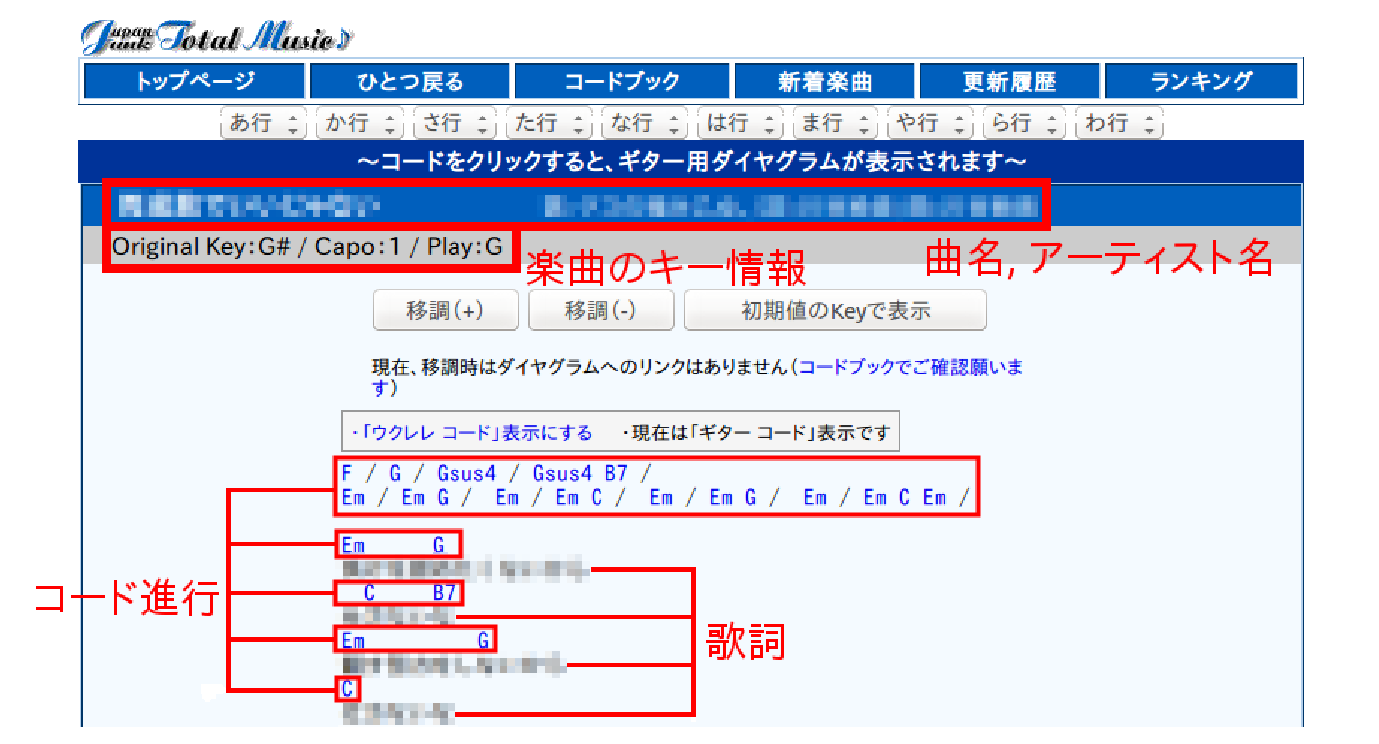
\includegraphics{jtm.eps}}
  \caption{楽曲データの例}
  \label{fig:jtm}
  \end{center}
\end{figurehere}

\section{コード進行による楽曲のモデル化}
本研究で構築したシステムにおける,
コード進行を用いた楽曲のモデル化に関する手法について述べる.
\subsection{コードの役割と特徴}
楽曲のコード進行を構成する各コードの役割は,
トニック, ドミナント, サブドミナントの3つに大きく分けられる.
以下にそれぞれの役割と特徴を示す.
\begin{description}
  \item[トニック (Tonic):]
    楽曲の調における主音のコードである.
    コード進行の起点や終点として用いられることが多く,
    一連のコード進行の中で聴覚的に安定した印象を与えるという役割を持つ.
    トニック, ドミナント, サブドミナントのどれにでも遷移しうるという特徴がある.
  \item[ドミナント (Dominant):]
    トニックに対して完全五度上にあるコードであり,
    一連のコード進行の中で聴覚的に不安定な印象を与えるという役割を持つ.
    安定を求めてトニックに遷移する確率が高いという特徴がある.
  \item[サブドミナント (Sub-Dominant):]
    トニックに対して完全五度下にあるコードである.
    ドミナントと同様に, 
    一連のコード進行の中で聴覚的に不安定な印象を与えるという役割を持つが,
    与える不安感はドミナントよりも小さい.
    トニック, ドミナントのどちらにも遷移しうるという特徴がある.
\end{description}

表\ref{tab:chords}にハ長調 (Cメジャー) の楽曲において主に利用される
各コードの役割を示す. 
なお, 
括弧付きで記述されているものはその構成音の類似性から
それぞれの役割を持つコードの代理として
利用されることが多いコードであることを意味している.
\vspace{-0.25cm}
\begin{tablehere}
  \begin{center}
  \caption{各コードの役割 (ハ長調)}
  \label{tab:chords}
  \begin{tabular}{c|c|c}
    \hline
    \hline
    役割 & 三和音 & 四和音 \\
    \hline
    T & C (Em, Am) & CM7 (C6, Em7, Am7) \\
    D & F (Dm) & FM7 (F6, Dm7) \\
    SD & G (Bm$^{-5}$) & G7 (Bm7$^{-5}$) \\
    \hline
    \hline
  \end{tabular}
  \end{center}
\end{tablehere}

\subsection{メジャーコードとマイナーコードの分類}
長調の楽曲において主音となるコードをメジャーコード,
短調の楽曲において主音となるコードをマイナーコードという.
一般的に,
メジャーコードは「明るい, 楽しい」といった印象を,
マイナーコードは「暗い, 悲しい」といった印象を与えることが多い.
コード進行を構成する各コードには様々なパターンがあるが,
本研究では楽曲のモデル化を簡易化するために代表的なコードのパターンを
メジャー/マイナーの2種類に分類した.
表\ref{tab:chord_class}に各コードの分類を示す.

\begin{tablehere}
  \begin{center}
  \caption{メジャー/マイナーコードの分類 (C)}
  \label{tab:chord_class}
  \begin{tabular}{|c|p{0.5\columnwidth}|}
    \hline
    メジャー & C, Csus4, Caug, C6, C7, CM7, C7sus4, C9 \\
    \hline
    マイナー & Cm, Cdim, Cm6, CmM7, Cm7, Cm7$^{-5}$ \\
    \hline
  \end{tabular}
  \end{center}
\end{tablehere}

\subsection{近親調}
楽曲を構成するコード進行を数値化する際に,
音楽理論において定義されている近親調 (関係調)\cite{NGSW07}を利用した.
近親調とは,
楽曲の調同士の類似性を定めるものである.
代表的な近親調の分類を以下に示す.
\begin{description}
  \item[同主調:]
    ハ長調 (Cメジャー) とハ短調 (Cマイナー) といった, 
    同じ主音を持つ2つの調の関係を意味する.
  \item[平行調:]
    ハ長調 (Cメジャー) とイ短調 (Aマイナー) といった,
    同一の調号を持つ2つの調の関係を意味する.
  \item[属調:]
    ハ長調 (Cメジャー) に対するト長調 (Gメジャー) といった,
    ある調とその完全五度上にある2つの調の関係を意味する.
  \item[下属調:]
    ハ長調 (Cメジャー) に対する ヘ長調 (Fメジャー) といった,
    ある調とその完全五度下にある2つの調の関係を意味する.
\end{description}

\subsection{コード進行の数値化}
近親調に基づいて類似している2つの調の主音は,
図\ref{fig:cof}に示す五度圏の上で近接した配置となる.
例として, ハ長調 (Cメジャー) を基準とした近親調について考える.
平行調となるイ短調 (Aマイナー), 
属調となるト長調 (Gメジャー),
下属調となるヘ長調 (Fメジャー)
はそれぞれハ長調 (Cメジャー) と隣接した位置にあるが,
同主調となるハ短調 (Cマイナー) は互いに直交した位置にある.
本研究では, 近親調に基づく主音同士の類似性と五度圏上での主音の位置関係を利用し,
コード進行の数値化を行なった.
例として,
「G, D, C, Bm, Em, G, Am, D」
というコード進行は
「1, 2, 0, 2, 1, 1, 0, 2」
として数値化される.

\begin{figurehere}
  \begin{center}
  \scalebox{0.3}{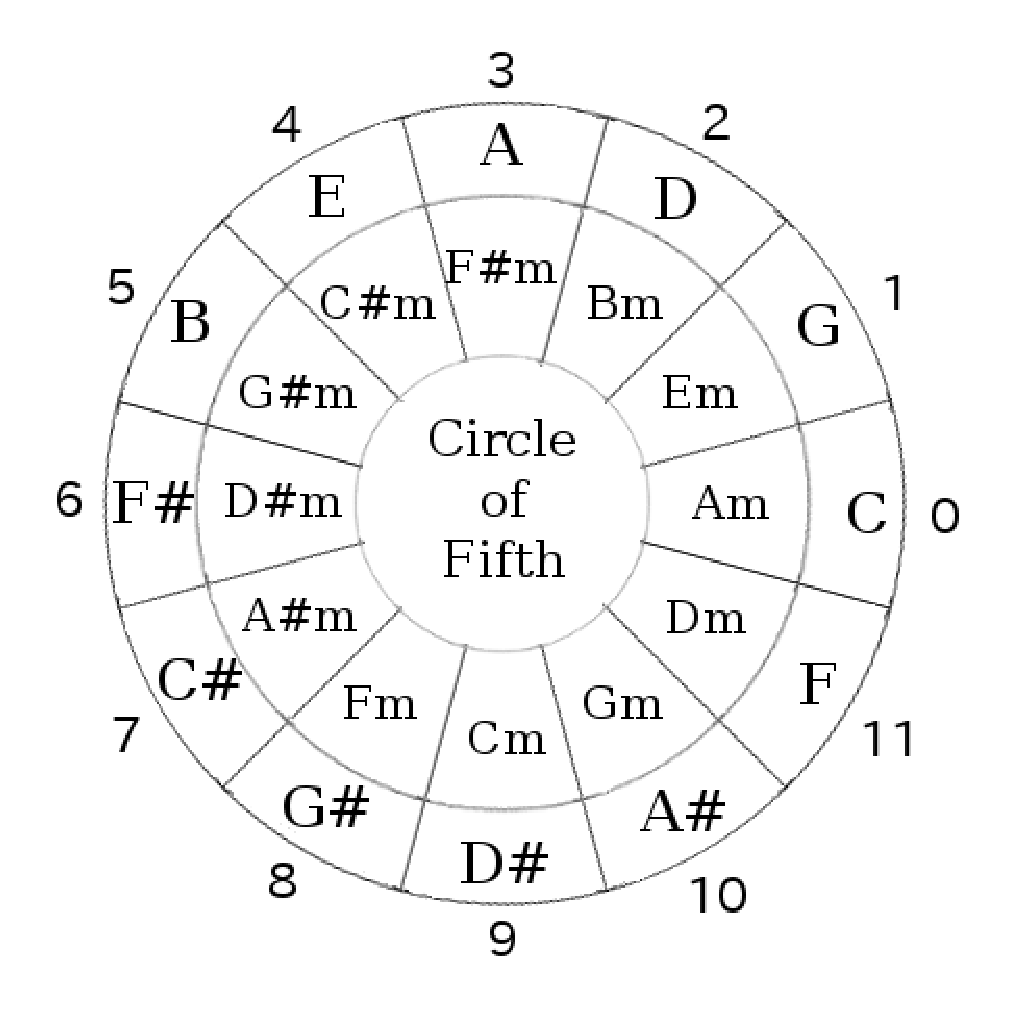
\includegraphics{cof.eps}}
  \caption{五度圏}
  \label{fig:cof}
  \end{center}
\end{figurehere}

\subsection{Hidden Markov Model}
コード進行に基づいて楽曲をモデル化するために
Hidden Markov Model (HMM)\cite{HMM} を利用した.
HMM は時系列で変化するデータを確率的にモデル化する手法であり,
入力データの変化を上手く表現することができるパラメータ
$\vector{\theta} = (\vector{\pi}, \vector{A}, \vector{B})$
を学習により求める.
ここで, 
$\vector{\pi}$ は初期状態確率,
$\vector{A}$ は状態遷移確率,
$\vector{B}$ はシンボル出力確率を意味する.
HMMのパラメータの学習法としては,
入力された時系列データからEMアルゴリズムにより
最適なパラメータを推定する
Baum-Welch アルゴリズム\cite{BWA}を利用した.

\subsection{HMM による楽曲のモデル化}
HMM はモデルのトポロジーを適切に設定することで,
対象とする問題に適した系列データのモデル化を行えるという特長を持つ.
本研究では,
楽曲のコード進行における各コードの役割が
トニック, ドミナント, サブドミナントという3つに大きく分けられるという点に着目し,
楽曲を図\ref{fig:hmm}に示す状態数3の Ergodic HMM によりモデル化した.

\begin{figurehere}
  \begin{center}
  \scalebox{0.4}{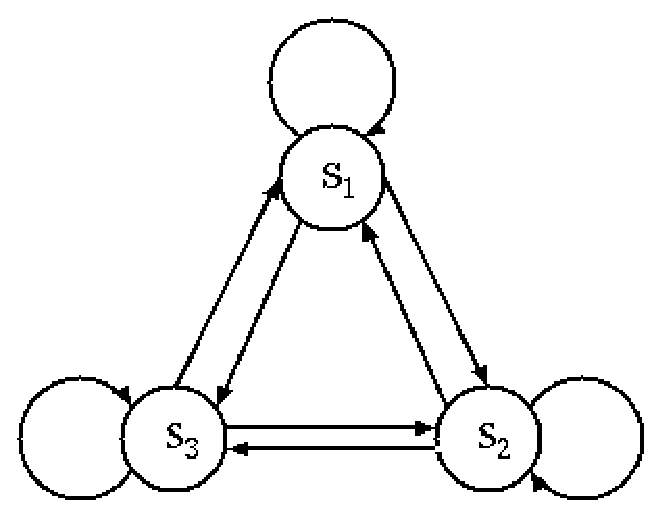
\includegraphics{hmm.eps}}
  \caption{Ergodic HMM のトポロジー}
  \label{fig:hmm}
  \end{center}
\end{figurehere}

コード進行に基づいて HMM による楽曲のモデル化を行う際,
HMM の各状態がそれぞれコードの役割 (T, D, SD) に対応する.
また, HMM の各パラメータはそれぞれ
\begin{description}
  \item[初期状態確率 $\vector{\pi}$:] 
    コード進行開始時のコード
  \item[状態遷移確率 $\vector{A}$:]
    コード遷移の様子
  \item[シンボル出力確率 $\vector{B}$:]
    コードの出現しやすさ
\end{description}
として対応付けされる.

\section{歌詞情報を用いた楽曲の印象分析}
本研究で構築したシステムにおける,
歌詞情報を利用した楽曲の印象分析に関する手法について述べる.
\subsection{Plutchik の感情の輪}
印象分析を行うための感情のモデルとして
Robert Plutchikにより提唱された「感情の輪」\cite{RP01} を用いた.
感情の輪は図\ref{fig:woe}に示すように,
感情を8つの基本感情 
(
"ecstasy", 
"admiration", 
"terror", 
"amazement", 
"grief", 
"loathing", 
"rage", 
"vigilance"
)
の強弱と組合せで表現するものである.
例として, 
"ecstasy" の基本感情の強度を弱めたものとして "joy" と "serenity" という感情があり,
"admiration" の基本感情の強度を弱めたものとして "trust" と "acceptance" という感情がある.
また, それぞれの基本感情を組み合わせたものとして "love" という感情があり,
これは "ecstasy" と "admiration" の基本感情が持つ性質
をそれぞれ半分ずつ持つ感情として考えられる.

\begin{figurehere}
  \begin{center}
  \scalebox{0.35}{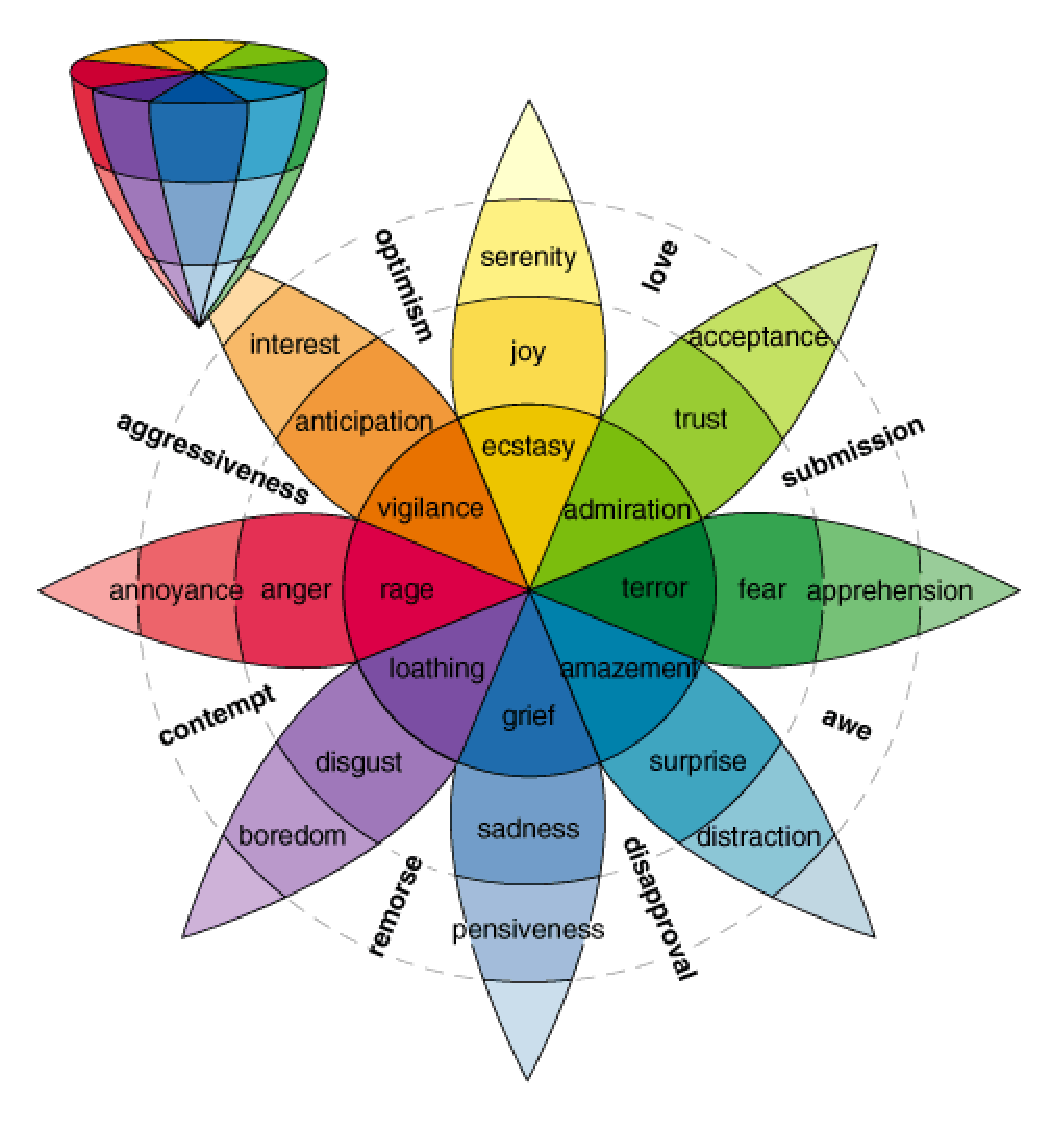
\includegraphics{woe.eps}}
  \caption{Plutchik の感情の輪}
  \label{fig:woe}
  \end{center}
\end{figurehere}

\subsection{感情スコアの定義}\label{subsec:a_score}
本研究では,
感情の輪に存在する英単語 (感情カテゴリ) に対し,
その位置に応じた感情スコアを8次元の数値ベクトルとして定義した.
数式で表現すると,
ある感情カテゴリ $c$ に対応する感情スコア $\mathrm{score}(c)$ は
\[
\mathrm{score}(c) =
(
s_{\mathrm{ecs}}, 
s_{\mathrm{adm}},
s_{\mathrm{ter}},
s_{\mathrm{ama}},
s_{\mathrm{gri}},
s_{\mathrm{loa}},
s_{\mathrm{rag}},
s_{\mathrm{vig}}
)
\]
として定義される.
$\mathrm{score}(c)$の各成分がそれぞれの基本感情の強度を意味する.
感情の輪の内側に存在する "ecstasy", "admiration" などの感情カテゴリは,
対応する感情スコアの成分が 1.0 となり,
1つ離れた "joy", "trust" などの感情カテゴリは,
対応する感情スコアの成分が 0.5 となる.
そして,
感情の輪の最も外側に位置している "serenity", "acceptance" などの感情カテゴリは,
対応する感情スコアの成分が 0.25 となる.
また,
"love" や "submission" といった2つの基本感情の組合せによって構成される
感情カテゴリは,
対応する感情スコアの成分の値をそれぞれ 0.5 ずつ持つものとして感情スコアを定義した.


\subsection{感情語辞書の作成}
楽曲の歌詞からの印象分析を行うために,
感情に関する語句 (感情語) を格納した感情語辞書を作成した.
感情語辞書は 
WordNet\cite{WN} および Thesaurus.com\cite{TS}
から得られた単語をもとにして作成しており,
感情カテゴリと類似した意味を持つ英単語
(下位語, 類義語, 派生系など) とその和訳を
含んでいる.
感情語の和訳を取得する際には日本語 WordNet\cite{JPNWN},
連想類語辞典\cite{RUIGO},
および Weblio 類語辞典\cite{WEBLIO}を利用した.
表\ref{tab:a_words}に感情語辞書に格納されている感情語の一例を示す.
例として,
「強い」という感情語を英訳したものは "strong" となり,
これは感情カテゴリにおける "trust" というカテゴリに属する感情語となる.

\begin{tablehere}
  \begin{center}
  \caption{感情語の一例}
  \label{tab:a_words}
  \begin{tabular}{ccc}
    \hline
    \hline
    感情語 & 英訳 & 感情カテゴリ \\
    \hline
    愛す & love & love \\
    言葉 & speech & interest \\
    強い & strong & trust \\
    \hline
    \hline
  \end{tabular}
  \end{center}
\end{tablehere}

\subsection{歌詞からの印象分析}
楽曲の歌詞に対して自然言語処理の手法を適用し,
その楽曲に対する印象分析を行なった.
以降に処理手順の概略を示す.

\subsubsection{感情語の抽出}
分類対象となる全ての楽曲の歌詞に対して係り受け解析を行い,
感情語を抽出する.
係り受け解析とは,
入力として与えられた文章を
その構成要素となる最小の単位 (形態素) の集合 (チャンク) に分解し,
各チャンクの修飾/非修飾の関係性を調査するための手法である.
本研究では,
形態素解析を行うための解析器として MeCab\cite{MeCab} を,
係り受け解析を行うための解析器として CaboCha\cite{CaboCha} をそれぞれ利用した.
例として,
「愛してるの言葉で僕は強くなれる」
という歌詞に対して係り受け解析を適用した結果を表\ref{tab:DP}に示す.

\begin{tablehere}
  \begin{center}
  \caption{係り受け解析の適用例}
  \label{tab:DP}
  \begin{tabular}{c|r|l}
    \hline
    \hline
    ID & 係り先 & 構成要素\\
    \hline
    0 & 1 & {愛し, てる, の}  \\
    1 & 4 & {言葉, で} \\
    2 & 4 & {僕, は} \\
    3 & 4 & {強く} \\
    4 & $-1$ & {なれる} \\
    \hline
    \hline
  \end{tabular}
  \end{center}
\end{tablehere}

表\ref{tab:DP}の解析結果をもとにして感情語辞書を参照し,
感情語辞書に含まれている単語を感情語として抽出する.
上記の例では
「愛す」, 「言葉」, 「強い」
という感情語が得られる.
なお,
係り受け解析結果の各チャンクにおける構成要素の中に
「〜ない」や「〜せず」といった否定表現が出現する場合は,
そのチャンクに含まれる感情語を抽出しないようにしている.
これは,
各感情語の意味を否定させた言葉が,
必ずしもその反対の感情を持つ言葉となるとは限らないと考えられるためである.

\subsubsection{感情スコアの算出}
抽出された感情語に対応する感情カテゴリを参照し,
それに基づいて各感情語に割り当てられる感情スコアを算出する.
前述の例に基づいて説明すると,
表\ref{tab:a_words}より,
「愛す」という感情語に対する感情カテゴリとして "love" が,
「言葉」という感情語に対する感情カテゴリとして "interest" が,
「強い」という感情語に対する感情カテゴリとして "trust" がそれぞれ得られる.
これらの感情カテゴリをもとに,
4.2節において前述した感情スコアの定義に基づいて
感情スコアを算出する.

\subsubsection{tf-idf による感情スコアの重み付け}
算出された感情スコアに対し,
tf-idf による重み付けを行う.
tf-idf は,
式 (\ref{eq:tf}) に示す tf (Term Frequency) と
式 (\ref{eq:idf}) に示す idf (Inverse Document Frequency) の積により,
文書中に出現する各単語に対して重み付けを行う手法である.
\begin{equation}\label{eq:tf}
\mathrm{tf}_{i, j} = \dfrac{n_{i, j}}{\sum_{k}n_{k, j}}
\end{equation}
\begin{equation}\label{eq:idf}
\mathrm{idf}_{i} = \mathrm{log}\dfrac{N}{N_{i}}
\end{equation}

ここで,
$n_{i, j}$ は単語 $word_{i}$ が文書 $doc_{j}$ の中に出現する回数,
$N$ は全文書の数,
$N_{i}$ は単語 $word_{i}$ が出現する文書の数をそれぞれ意味する.
tf-idf による重み付けを行うことにより,
1つの文書に多く出現する単語に対して大きな重みを,
複数の文書に渡って多く出現する単語に対して小さな重みを割り当てることが可能となる.
そのため,
1つの楽曲の中で繰り返し出現するような感情語に対する感情スコアの重みは大きくなり,
「愛す」や「好き」などといった
複数の楽曲の歌詞で多く出現することが予想される
感情語に対する感情スコアの重みは小さくなる.

\section{教師なし学習による楽曲分類}
本研究で構築したシステムにおける,
教師なし学習を用いた楽曲分類に関する手法について述べる.
\subsection{楽曲の特徴量}
3節で述べたコード進行の分析により得られたコード進行に関する特徴量
(HMM のパラメータ) と,
4節で述べた歌詞情報の分析により得られた楽曲に対する感情スコア
(8次元の数値ベクトル) に基づき,
楽曲の特徴空間を構成した.
本研究では状態数3, 出力シンボル数12の Ergodic HMM を利用しているため,
初期状態確率 $\vector{\pi}$ は3次元のベクトル,
状態遷移確率 $\vector{A}$ は $(3 \times 3)$ の行列,
シンボル出力確率 $\vector{B}$ は $(12 \times 3)$ の行列となる.
そのため,
構成される楽曲の特徴空間の次元は合計で56となる.

\subsection{$k$-means++ 法}
楽曲の分類を行うための手法として $k$-means++ 法\cite{KMPP}を利用した.
$k$-means++ 法は
代表的な教師なし学習アルゴリズムの一つとして知られている
$k$-means 法\cite{KMEANS}を改良した手法である.
$k$-means 法は各データに対する初期クラスタ番号をランダムに割り当てるため,
初期クラスタの選び方によって大きく性能が変化しうるという欠点がある.
それに対し, $k$-means++ 法では
初期クラスタの中心を重み付けされた確率分布から選択するため,
分類開始時における初期クラスタの中心を
できる限り遠くに離すことが可能となる.

\section{分類実験とその結果}
本研究で構築した楽曲分類システムを評価するために行なった
楽曲の分類実験およびその結果について述べる.

\subsection{実験の概要}
J-Total Music における
累計人気楽曲ランキングから参照した計300曲の楽曲データを利用し,
本研究で構築したシステムによる楽曲分類実験を行なった.
表~\ref{tab:rank}に実験対象とした楽曲データの一例を示す.
なお, 
$k$-means++ 法により分類を行う際に指定する必要があるクラスタ数は,
本研究では五度圏上に存在する全ての主音の個数である24とした.

\begin{tablehere}
  \begin{center}
  \caption{累計人気楽曲ランキング (上位5曲)}
  \label{tab:rank}
  \begin{tabular}{c|r|r}
    \hline
    \hline
    順位 & 曲名 & アーティスト名 \\
    \hline
    1 & チェリー & スピッツ \\
    2 & 粉雪 & レミオロメン \\
    3 & 空も飛べるはず & スピッツ \\
    4 & 3月9日 & レミオロメン \\
    5 & ロビンソン & スピッツ \\
    \hline
    \hline
  \end{tabular}
  \end{center}
\end{tablehere}

\subsection{分類実験の結果}
図\ref{fig:cls1}および図\ref{fig:cls2}に
分類結果として実際に構成された2つのクラスタを示す.
以降,
図\ref{fig:cls1}に示す結果として構成されたクラスタをクラスタ1,
図\ref{fig:cls2}に示す結果として構成されたクラスタをクラスタ2
とそれぞれ称する.

\begin{figurehere}
  \begin{center}
  \scalebox{0.2}{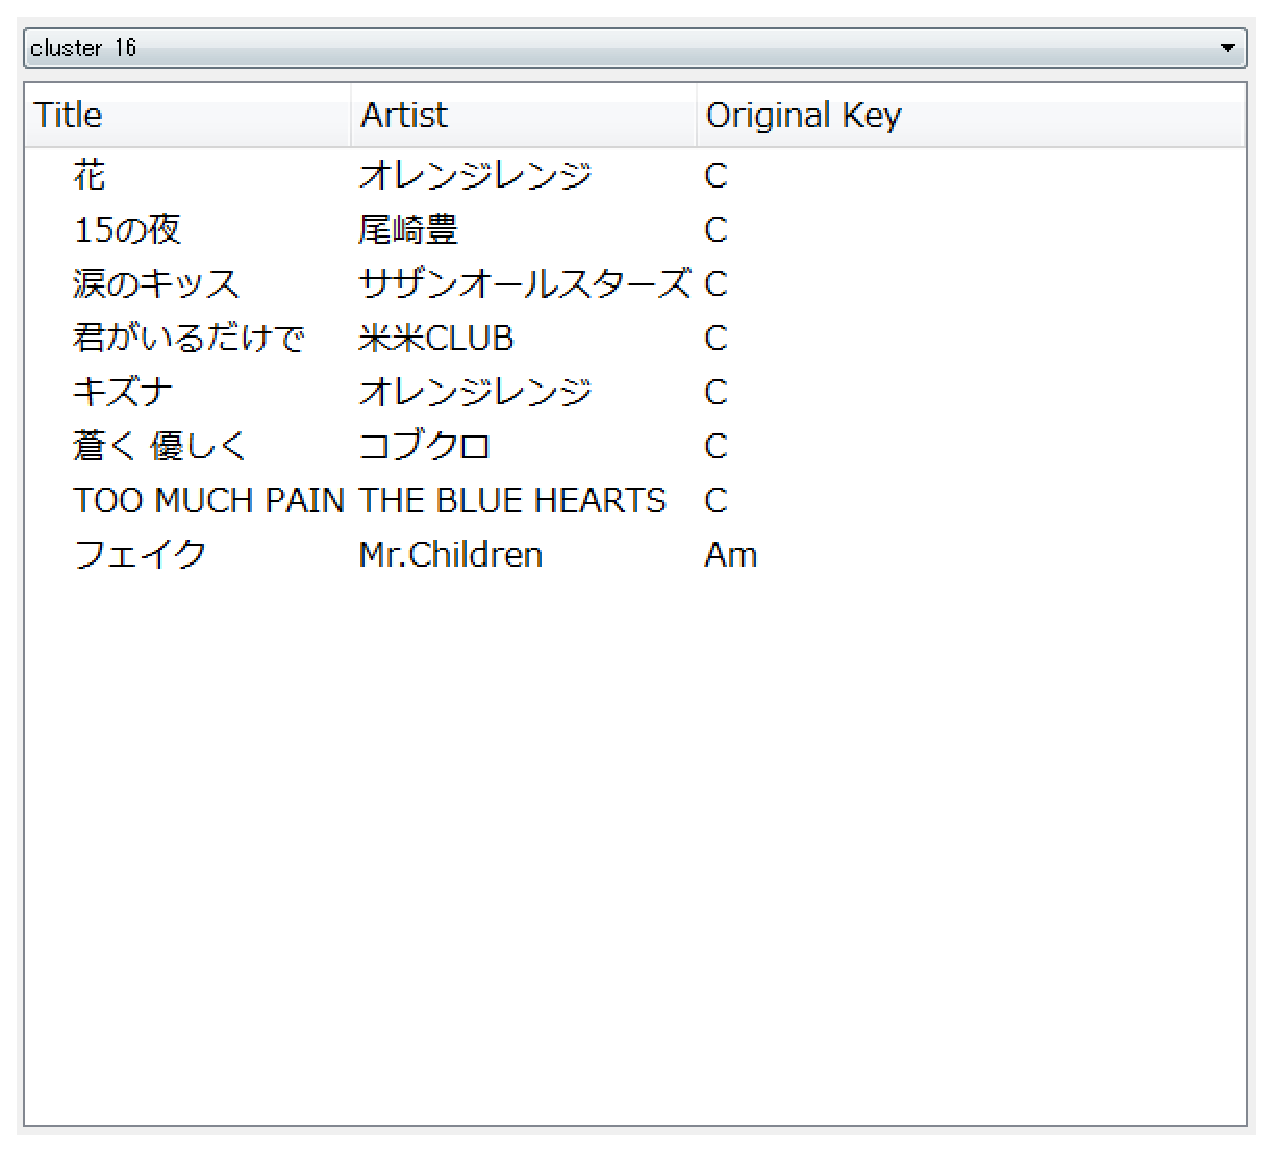
\includegraphics{cls1.eps}}
  \caption{分類結果 (クラスタ1)}
  \label{fig:cls1}
  \end{center}
\end{figurehere}
\begin{figurehere}
  \begin{center}
  \scalebox{0.2}{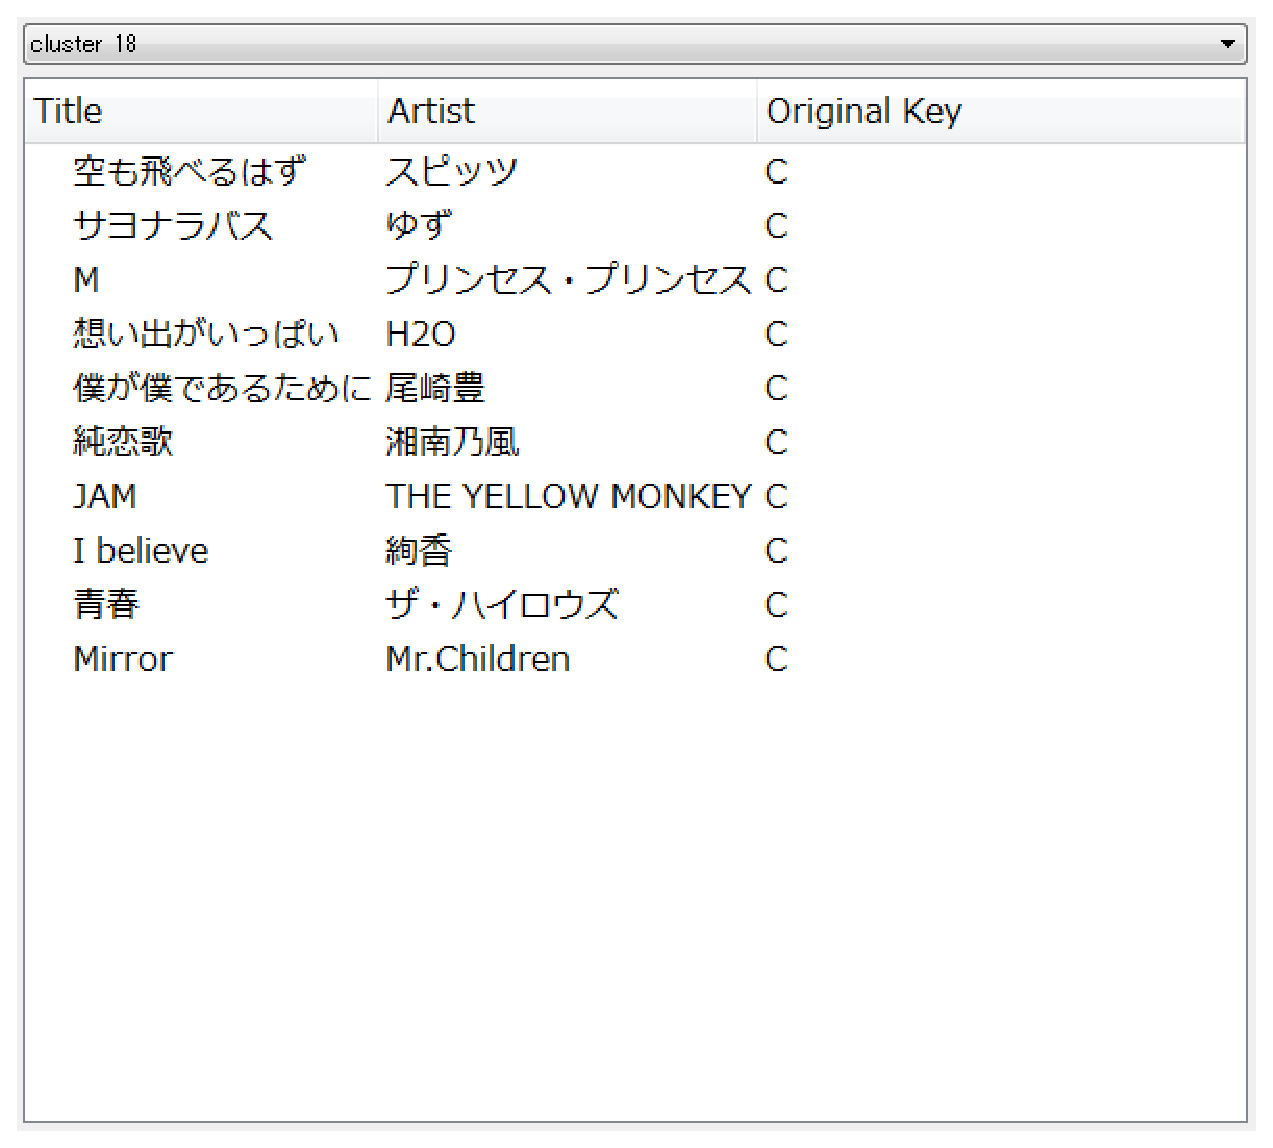
\includegraphics{cls2.eps}}
  \caption{分類結果 (クラスタ2)}
  \label{fig:cls2}
  \end{center}
\end{figurehere}

次に,
クラスタ1に含まれる楽曲に対して
印象分析を行なった結果を図\ref{fig:emo1}に,
クラスタ2に含まれる楽曲に対して
印象分析を行なった結果を図\ref{fig:emo2}にそれぞれ示す.

\begin{figurehere}
  \begin{center}
  \scalebox{0.2}{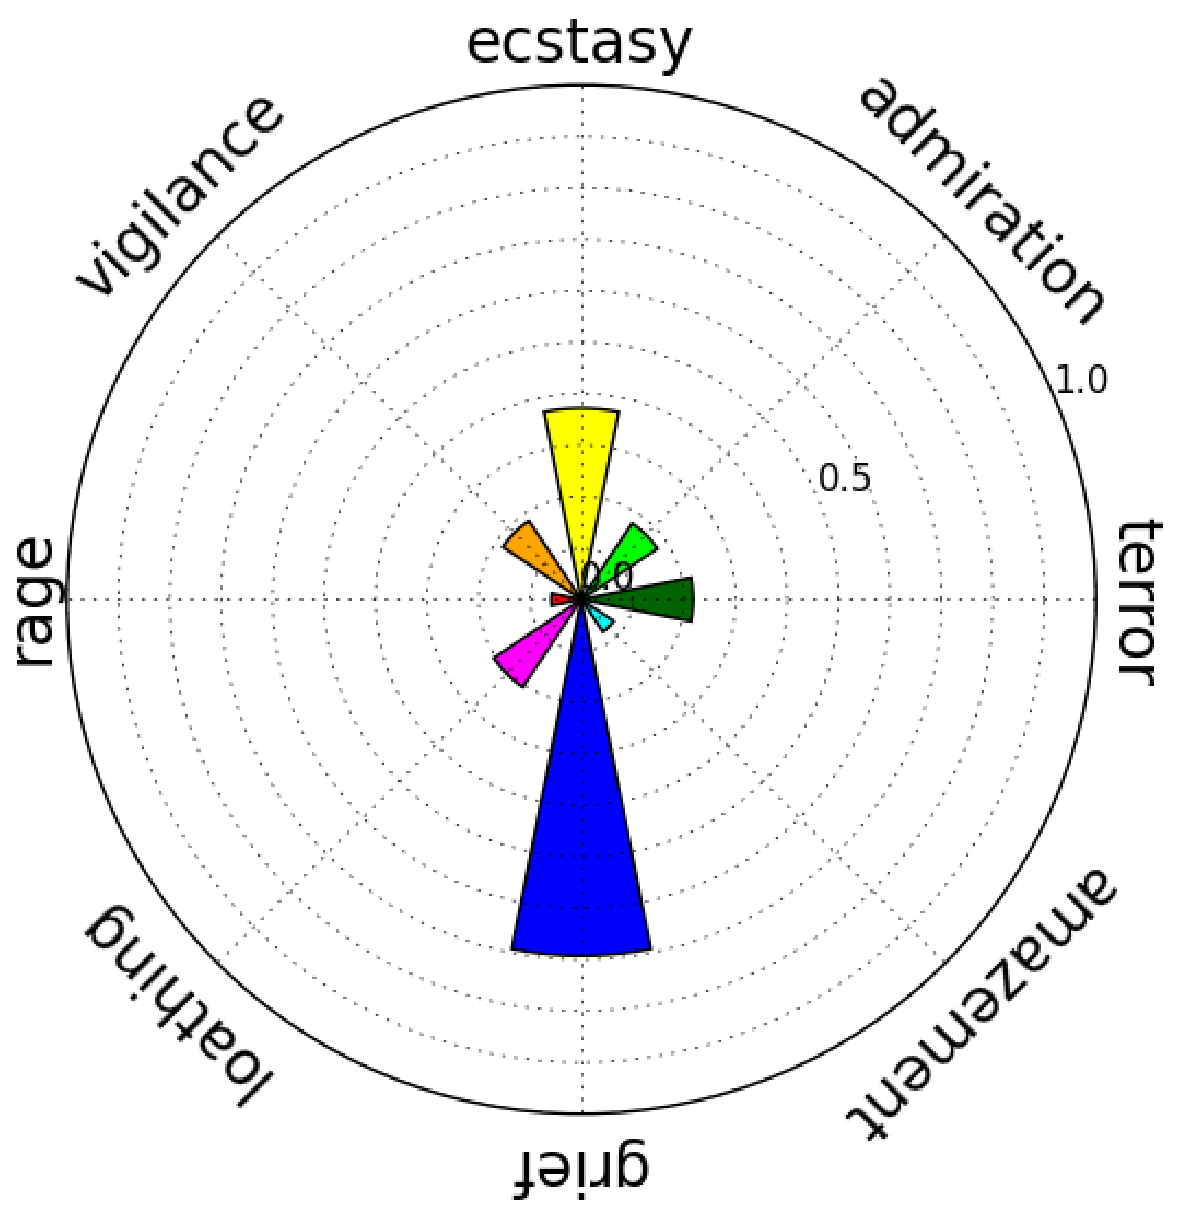
\includegraphics{emo1.eps}}
  \caption{印象分析結果 (クラスタ1)}
  \label{fig:emo1}
  \end{center}
\end{figurehere}
\begin{figurehere}
  \begin{center}
  \scalebox{0.2}{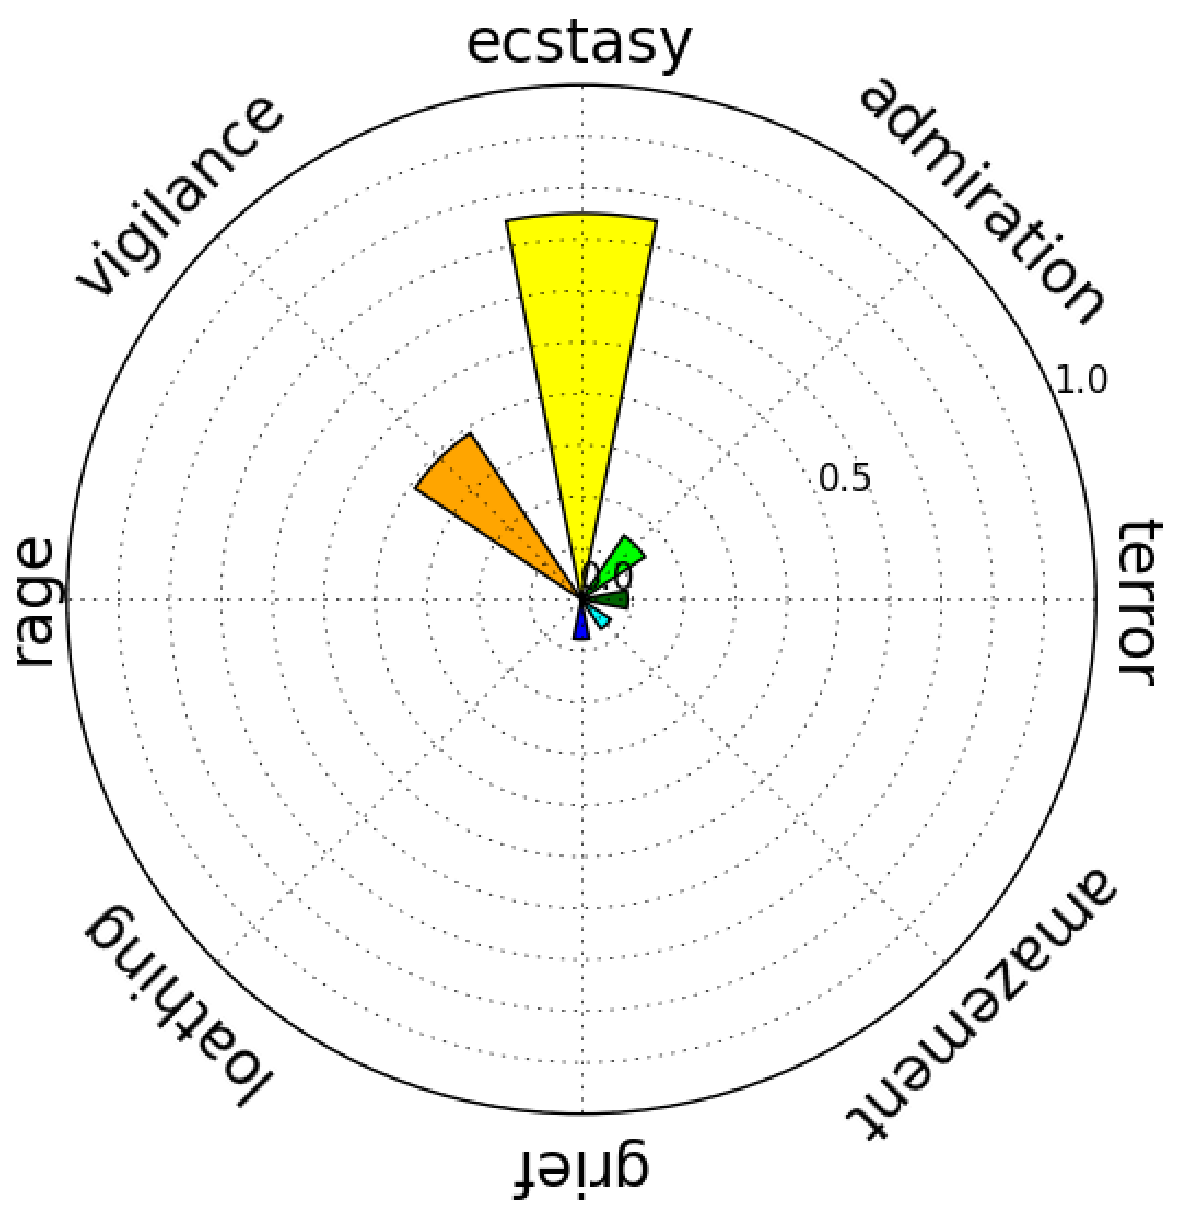
\includegraphics{emo2.eps}}
  \caption{印象分析結果 (クラスタ2)}
  \label{fig:emo2}
  \end{center}
\end{figurehere}

\subsection{実験結果の考察}
図\ref{fig:cls1}および図\ref{fig:cls2}に示す2つのクラスタは,
どちらもほぼ全て原曲キーをCメジャーとする楽曲の集合として構成されている.
しかし,
各クラスタに含まれる楽曲に対する印象分析の結果を検証したところ,
クラスタ1は
図\ref{fig:emo1}に示す結果のように "grief" の感情スコアが高い楽曲を多く含んでおり,
クラスタ2は
図\ref{fig:emo2}に示す結果のように "ecstasy" の感情スコアが高い楽曲を多く含んでいることが確認された.
これらの結果より,
本研究で構築したシステムは
曲調の類似性だけでなく,
楽曲に対する印象の類似性も反映させた分類を行なっていることが推測される.

今回の実験ではクラスタ数を24とした楽曲の分類を行い,
その結果として各クラスタが曲調的に概ね
類似している楽曲の集まりとして構成されていることが確認された.
しかし,
現時点では
分類の際に曲調の類似性と歌詞に基づく印象の類似性のどちらを重視するかを
考慮していない.
そのため,
今後は分類を行う際に
曲調の類似性 (コード進行から得られた特徴量) と
印象の類似性 (歌詞から得られた特徴量) に対する重み付けをユーザが指定できるようにする
必要があると考えられる.
また, 
実際にヒット曲や各ユーザが好む楽曲を分類する際には,
各楽曲の曲調や印象に対して偏りが生じることも予想されるため,
楽曲分類を行う際の適切なクラスタ数についても
さらに検証を進める必要があると考えられる.

\section{おわりに}
本研究では, 
楽曲のコード進行に関する情報を HMM により分析し,
歌詞に関する情報を用いて楽曲に対する印象を推定する機能を持つシステムを構築した.
また, 
コード進行と歌詞情報の双方の分析結果を利用した楽曲分類実験を行い,
その結果として
本研究で構築したシステムが曲調および印象を考慮した楽曲の分類を行うことを確認した.

今後の展望としては,
歌詞に基づく楽曲の印象分析の結果を利用した楽曲検索を行う機能などの追加により,
より実用的な楽曲分類および分析を行うシステムの実現を目指す.
また,
実際に曲調や印象などをユーザから聴取した楽曲データを用いた分類実験を行い,
本研究で構築したシステムの定量的な評価を行う.

\section{謝辞}
本研究を進めるにあたり,
様々な面からご指導, ご助言, ご支援を頂いた,
釧路高専情報工学科所属の天元宏准教授に深く感謝し御礼申し上げます.
また, 
研究室での日々を共に過ごした天元研究室の同輩の皆様,
ならびに釧路高専専攻科での2年間を共にした皆様に厚く御礼申し上げます.

%
% 以下に文献を書きます。
%

{\small
\begin{thebibliography}{99}
  \bibitem{NGSW07}
    長澤 槙子, 渡辺 知恵美, 伊藤 貴之, 増永 良文, 
    “近親調を用いた楽曲クラスタリングシステムの構築に向けて”,
    電子情報通信学会第18回データ工学ワークショップ論文集, 2007.
  \bibitem{FNSW09}
    舟澤 慎太郎, 石先 広海, 帆足 啓一郎, 滝嶋 康弘, 甲藤 二郎,
    “歌詞の印象に基づく楽曲検索のための楽曲自動分類に関する検討”,
    情報処理学会第71回全国大会講演論文集, 2009.
  \bibitem{JTM}
    J-Total Music, “http://music.j-total.net/”
  \bibitem{HMM}
    Z. Ghahramani,
    “\textit{An Introduction to Hidden Markov Models and Bayesian Networks}”,
    International Journal of Pattern Recognition and Artificial Intelligence,
    Vol. 15, No. 9, pp. 9-42, 2001.
  \bibitem{BWA}
    L. E. Baum, T. Petrie, G. Soules, and N. Weiss,
    “\textit{A Maximization Technique Occurring in the Statistical Analysis of Probabilistic Functions of Markov Chains}”,
    The Annals of Mathematical Statistics, Vol. 41, No. 1, pp. 161-171,
    1970.
  \bibitem{RP01}
    R. Plutchik,
    “\textit{The Nature of Emotions}”,
    American Scientist, Vol. 89, No. 4, pp. 344-350, 2001.
  \bibitem{WN}
    WordNet, “https://wordnet.princeton.edu/”
  \bibitem{TS}
    Thesaurus.com, “http://www.thesaurus.com/”
  \bibitem{JPNWN}
    日本語 WordNet, “http://nlpwww.nict.go.jp/wn-ja/”
  \bibitem{RUIGO}
    連想類語辞典, “http://renso-ruigo.com/”
  \bibitem{WEBLIO}
    Weblio 類語辞典, “http://thesaurus.weblio.jp/”
  \bibitem{MeCab}
    T. Kudo, K. Yamamoto, and Y. Matsumoto,
    “\textit{Applying Conditional Random Fields to Japanese Morphological Analysis}”,
    Proc. of the 2004 Conference on Empirical Methods in Natural Language Processing, pp. 230-237, 2004.
  \bibitem{CaboCha}
    工藤 拓, 松本 裕治, 
    “チャンキングの段階適用による日本語係り受け解析”,
    情報処理学会論文誌, Vol. 43, No. 6, 2002.
  \bibitem{KMPP}
    D. Arthur and S. Vassilvitskii,
    “\textit{k-means++: The Advantages of Careful Seeding}”,
    Proc. of the eighteenth annual ACM-SIAM Symposium on Discrete Algorithms, pp. 1027-1035, 2007.
  \bibitem{KMEANS}
    S. P. Lloyd.
    “\textit{Least Squares Quantization in PCM}”,
    IEEE Transactions on Information Theory, Vol. 28, No. 2, pp. 129-138, 1982.
\end{thebibliography}
}

\end{multicols}
\end{document}
